\documentclass{article}

% if you need to pass options to natbib, use, e.g.:
% \PassOptionsToPackage{numbers, compress}{natbib}
% before loading nips_2017
%
% to avoid loading the natbib package, add option nonatbib:
% \usepackage[nonatbib]{nips_2017}
\PassOptionsToPackage{numbers, compress}{natbib}
\usepackage{nips_2017}

% to compile a camera-ready version, add the [final] option, e.g.:
% \usepackage[final]{nips_2017}

\usepackage[utf8]{inputenc} % allow utf-8 input
\usepackage[T1]{fontenc}    % use 8-bit T1 fonts
\usepackage{hyperref}       % hyperlinks
\usepackage{url}            % simple URL typesetting
\usepackage{booktabs}       % professional-quality tables
\usepackage{amsmath}
\usepackage{amsfonts}       % blackboard math symbols
\usepackage{nicefrac}       % compact symbols for 1/2, etc.
\usepackage{microtype}      % microtypography
\usepackage{graphicx}
\usepackage{caption}
\usepackage{subcaption}
\bibliographystyle{unsrtnat}

\title{Bayesian Inference of Plasma Diffusion Parameters: An LSSVM based approach}

% The \author macro works with any number of authors. There are two
% commands used to separate the names and addresses of multiple
% authors: \And and \AND.
%
% Using \And between authors leaves it to LaTeX to determine where to
% break the lines. Using \AND forces a line break at that point. So,
% if LaTeX puts 3 of 4 authors names on the first line, and the last
% on the second line, try using \AND instead of \And before the third
% author name.

\author{
  Mandar H.~Chandorkar\thanks{mandar2812.github.io} \\
  Multiscale Dynamics\\
  Centrum Wiskunde Informatica\\
  Amsterdam 1098XG, the Netherlands\\
  \texttt{mandar.chandorkar@cwi.nl} \\
  %% examples of more authors
   \And
   Enrico ~Camporeale \\
   Multiscale Dynamics \\
   Centrum Wiskunde Informatica \\
   \texttt{e.camporeale@cwi.nl} \\
   \AND
   Cyril \\
   Furthlener \\
   INRIA, Paris-Saclay \\
   \texttt{furthlen@inria.fr} \\
   \And
   Michele Sebag \\
   INRIA, Paris-Saclay \\
   \texttt{sebag@inria.fr} \\
  %% \And
  %% Coauthor \\
  %% Affiliation \\
  %% Address \\
  %% \texttt{email} \\
}

\begin{document}
% \nipsfinalcopy is no longer used

\maketitle

\begin{abstract}
  The abstract paragraph should be indented \nicefrac{1}{2}~inch
  (3~picas) on both the left- and right-hand margins. Use 10~point
  type, with a vertical spacing (leading) of 11~points.  The word
  \textbf{Abstract} must be centered, bold, and in point size 12. Two
  line spaces precede the abstract. The abstract must be limited to
  one paragraph.
\end{abstract}

\section{Introduction}

\section{Methodology}

Bayesian inference involves specifying the following components.
\begin{enumerate}
\item Prior distribution over system parameters.
\item Quantification of likelihood over observations.
\item Procedure for performing inference, i.e. exact inference, \emph{Markov Chain
    Monte Carlo}, \emph{Variational methods}, etc.
\end{enumerate}

Performing Bayesian inference over parameters of physical systems,
involves synthesizing pre-exsiting knowledge of the physical system in
question i.e. the \emph{partial differential equation} (PDE), with
statistical techniques. The aim of such an exercise is often the
quantification of uncertainty over system parameters from an often
sparse set of observations which are quantities of interest in the
physical system. 

\subsection{Inverse Problems}\label{sec:inv}

The \emph{inverse problem} can be stated as follows: given a set of
noisy observations $y$ scattered in the space time domain, of a
physical quantity $f$ governed by the dynamical system
$\mathcal{L}_{\theta} f = Q_{\theta}$, estimate the parameters $\theta$ of the
dynamical system $(\mathcal{L}_{\theta}, Q_{\theta})$.

In this formalism $\mathcal{L}_{\theta}$ is a differential operator,
$Q_{\theta}$ is a \emph{source term} and $\theta$ is a collection of parameters
which specify the operator and the source term.

\subsection{Physical System: Plasma Diffusion}

The radial diffusion system is a simplified one-dimensional version of
the \emph{Fokker-Plank} equation. It tracks the time evolution of the
\emph{phase space density} of particles, $f$ which is goverened by the
differential equation \ref{eq:raddiffusion} known as \emph{radial
  diffusion} \citep{JGRA:JGRA9345}.

\begin{equation}\label{eq:raddiffusion}
  \frac{\partial{f}}{\partial{t}} = l^2 \frac{\partial}{\partial{l}}\left( \frac{\kappa(l,
      t)}{l^{2}} \frac{\partial{f}}{\partial{l}} \right) - \lambda(l,
  t) f +  Q(l, t)
\end{equation}

The \emph{phase space density}, $f$, is a function of the spatial
coordinate $l$ which is also known as the \emph{Roederer} $L^*$ or
\emph{L-shell} in magnetospheric physics \citep{Roederer1970}.

The key quantities in the system above are.

\begin{enumerate}
\item $f$: The density of particles as a function of space $l$ and
  time $t$.
\item $\kappa(l, t)$: Diffusion field.
\item $\lambda(l, t)$: Loss rate, this is a non-negative
  quantity which indicates how quickly particles are lost from the
  radiation belts.
\item $Q(l, t)$: Particle injection rate.
\end{enumerate}

Casting system \ref{eq:raddiffusion} in terms of the terminology of
section \ref{sec:inv}, $\mathcal{L}_{\theta} =
\frac{\partial}{\partial{t}} - l^2 \frac{\partial}{\partial{l}}\left( \frac{\kappa(l,
      t)}{l^{2}} \frac{\partial}{\partial{l}} \right) - \lambda(l,
  t)$. In this case $\theta$ would a collection of parameters which
  would specify the analytic expressions for $\kappa(l,t)$,
  $\lambda(l,t)$ and $Q(l,t)$.

\subsubsection*{Diffusion Parameters}

To solve the radial diffusion system \ref{eq:raddiffusion}, the
quantities $\kappa(l, t)$, $\lambda(l, t)$ and $Q(l, t)$ need to be
specified. It is a common practice (see \citet{GRL:GRL10762},
\citet{JGRA:JGRA15067}, \citet{JGRA:JGRA18021} and
\citet{GRL:GRL22815}) to parameterise the diffusion field
$\kappa$ and loss rate $\lambda$ in the following manner.

\begin{align}
  \kappa(l,t), \lambda(l, t) \sim \alpha l^{\beta} 10^{b Kp(t)} \\
\end{align}

The quantities $\alpha$, $\beta$ and $b$ are parameters which define
the diffusion field and loss rate while the quantity $Kp(t)$ is known
as the Kp index, a measured quantity which stands as a proxy for the
global geomagnetic activity \cite{BartelsKp}.

\subsection{Model Formulation}

We approach the radial diffusion inference problem by formulating a
modified version of the \emph{least squares support vector machine}
predictor for obtaining a closed form approximation to the phase space
density $f$ which tries to satisfy the radial diffusion PDE
\ref{eq:raddiffusion} on a fixed set of \emph{colocation} points while
minimising error on a set of sparse noisy observations. 
Using the surrogate phase space density estimator as a baseline, we
specify the likelihood of the observations.

\emph{Least Squares Support Vector Machines}(LSSVM) have been applied
to calculating approximate solutions to PDEs
\citep{MEHRKANOON2015105}, \citep{MEHRKANOON20122502} as well as
parameter estimation of delay differential equations
\citep{MEHRKANOON2014830}, the approach taken in the aforementioned
research (\citet{MEHRKANOON2014830}) was expressing the parameter
estimation of time delay as an algebraic optimization problem
resulting in closed-form approximation for the time varying parameters
while avoiding iterative simulation of the dynamical system (governed
by the delay differential equations) in the parameter estimation process.

\subsubsection*{Surrogate Phase Space Density Model}

Let $\mathcal{D}={(x^{o}_{i}, y_{i}): i = 1 \cdots n_{o}}$ be a set of
noisy observations of the phase space density $f$, where $x_{i} =
(l_{i}, t_{i})$ are points in the space time domain. We seek a linear
estimator for $f$ of the form $\hat{f}(x) = w^{T}\varphi(x) + b$,
where $\varphi(.): \mathbb{R}^{2} \rightarrow \mathbb{R}^{d}$ is a $d$
dimensional feature map and $b$ is a scalar intercept.

Further let $\mathcal{C} ={(x^{o}_{i}, y_{i}): i = 1 \cdots n_{o}}$ be 
a set of colocation points on which we aim to enforce radial diffusion
dynamics.

We exploit the linearity of the differential operator
$\mathcal{L}_{\theta}$ and note that $\mathcal{L}_{\theta} [\hat{f}(x)]
= w^{T} \mathcal{L}_{\theta}[\varphi(x)]$, yielding an estimator
$\hat{Q}(x) = w^{T}\psi(x)$ where $\psi_{\theta}(x) =
\mathcal{L}_{\theta}[\varphi(x)]$. Calculating $w \in \mathbb{R}^d$
can now be cast as the following constrained $L_2$ regularized 
least squares problem.

\begin{align}\label{eq:surrogate}
   min_{w,e,\epsilon} \ \mathcal{J}(w,e,\epsilon;\theta) &= 
   \frac{1}{2} w^{T}w + \frac{1}{2\gamma_{o}} \sum_{k = 1}^{n_{o}}{e^{2}_{k}} + \frac{1}{2\gamma_{c}} \sum_{k = 1}^{n_{c}}{\epsilon^{2}_{k}} \\
  & s.t \nonumber \\
  y_{i} & = w^{T}\varphi(x^{o}_{i}) + b + e_{i}, \ \ i = 1 \cdots n_{o} \\
  q_{i} & = w^{T}\psi_{\theta}(x^{c}_{i}) + \epsilon_{i}, \ \ i = 1 \cdots n_{c}
\end{align}

It can be seen that system \ref{eq:surrogate} is similar to the
formulation of the LSSVM model, while incorporating the dynamics of
linear PDE systems into its loss function. 

The quantities $\gamma_{o}$ and $\gamma_{c}$ are weights attached to
the errors on observations and colocation points respectively, thus
by smoothly varying them one may assign higher or lower importance for
the surrogate model to fit the observational data and the dynamics of
the physical system.

In order to solve this system one must construct its
\emph{Lagrangian}.

\begin{align*}\label{eq:lag}
      \mathfrak{L}(w,e,\epsilon, \alpha_{1 \cdots k}, \beta_{1 \cdots k}; \theta; \gamma_{o}; \gamma_{c}) &= 
      \frac{1}{2} w^{T}w + \frac{1}{2\gamma_{o}} \sum_{k = 1}^{n_{o}}{e^{2}_{k}} +
      \frac{1}{2\gamma_{c}} \sum_{k = 1}^{n_{c}}{\epsilon^{2}_{k}} \\
      & + \sum_{k = 1}^{n_{o}}{\alpha_{k}(y_{k} - w^{T}\varphi(x^{o}_{k}) + b + e_{k})} \\
      & + \sum_{k = 1}^{n_{c}}{\beta_{k}(q_{j} - w^{T}\psi_{\theta}(x^{c}_{j}) + \epsilon_{j})} 
\end{align*}

Given fixed values for $\gamma_{o}$, $\gamma_{c}$ and PDE parameters
$\theta$, the equation above expresses the Lagrangian of system
\ref{eq:surrogate}. The quantities $\alpha_{1}, \cdots, \alpha_{n_{o}}$ and
$\beta_{1}, \cdots, \beta_{n_{c}}$ are the \emph{Lagrange multipliers}
introduced for equality constraints of the system. Applying the
\emph{Karush-Kuhn-Tucker}(KKT) conditions the solution of the
optimization problem \ref{eq:surrogate} can be expressed in terms of
the Lagrange multipliers $\alpha = (\alpha_{1}, \cdots, \alpha_{n_{o}})$
$\beta = (\beta_{1}, \cdots, \beta_{n_{c}})$.

\begin{equation}\label{eq:solution}
  \begin{bmatrix}
    0 & \mathbf{1}^{T} & \mathbf{0} \\ 
    \mathbf{1} & \Omega + \gamma_{o}I  & \Omega_*\\ 
    \mathbf{0} & \Omega_{*}^{T}  & \Omega_{**} + \gamma_{c}I 
  \end{bmatrix} \begin{bmatrix}
    b\\ 
    \alpha\\ 
    \beta
  \end{bmatrix} = \begin{bmatrix}
    0\\ 
    y\\ 
    q
  \end{bmatrix}
\end{equation}

The components of the symmetric block matrix system on the left hand side of 
\ref{eq:solution} are 
\begin{enumerate}
\item $\Omega \in \mathbb{R}^{n_{o} \times n_{o}}: \omega_{ij} = \varphi(x^{o}_{i})^{T} \varphi(x^{o}_{j})$
\item $\Omega_{**} \in \mathbb{R}^{n_{c} \times n_{c}}: \omega^{**}_{ij} = \psi(x^{c}_{i})^{T} \psi(x^{c}_{j})$
\item $\Omega_{*} \in \mathbb{R}^{n_{o} \times n_{c}}: \omega^{*}_{ij} = \varphi(x^{o}_{i})^{T} \psi(x^{c}_{j})$
\end{enumerate}

The surrogate model can now be used to estimate the phase space density 
at a point $x = (l,t)$.

\begin{equation}\label{eq:model}
\hat{f}(x;\theta) = \sum_{k = 1}^{n_{o}}{\alpha_{k}\varphi(x)^{T}\varphi(x^{o}_{k}) + \sum_{k = 1}^{n_{c}}}{\beta_{k} \varphi(x)^{T} \psi_{\theta}(x^{c}_{k})} + b
\end{equation}

\subsection*{Choice of Basis}

There exist several choices regarding the basis $\varphi(.)$, they are but not limited to 
orthogonal polynomials, Fourier series, radial basis functions etc. 

Radial basis functions were first applied for solution of PDE problems in \cite{KANSA1990147}, 
the authors used colocation with \emph{multiquadric} basis functions for approximating solutions
of boundary value problems.

Radial basis functions have been applied for the mesh-free solutions of Poisson PDE systems 
(\citep{AMINATAEI20082887}, \citep{DUAN200866}, \citep{DUAN2006394} \& \citep{CNM:CNM419}),
as well as the Poisson control problem \citet{Pearson2013}. Further applications of RBFs include 
atmospheric flow \citep{Tillenius2015406}, convection-diffusion \citep{Safdari-Vaighani2015}, and 
Schrödinger's equation (\citep{doi:10.1137/120893975}, \citep{doi:10.1063/1.3637863}). 

For our problem we choose a basis which is a product of a multiquadric radial basis in space and 
an inverse multiquadric basis in time.

\begin{equation}\label{eq:basis}
\varphi_{i}(l,t) = \frac{\sqrt{1+(|l - l_{i}|/\rho_{l})^{2}}}{(1+(|t - t_{i}|/\rho_{t})^{2})^{s/2}}
\end{equation}

The nodes of the basis are placed on a regular rectangular grid and their 
length scales $\rho_l$ and $\rho_t$ are set to the distance between adjacent
node points. The value of the exponent $s$ in equation \ref{eq:basis} should be
a positive value between $0$ and $1$, we observe that setting $s = 0.75$ works well
in practice.

\subsubsection*{Quantifying Observation Likelihood}

We assume a multivariate Gaussian distribution for calculating the likelihood of 
the observations conditioned on the system parameters $\theta$. 

The surrogate model \ref{eq:model} gives a baseline or mean value for the phase space density, we use a
hybrid RBF covariance function $C(x_{i}, x_{j}) = \sigma^2 exp(-\frac{1}{2} (\frac{|l_i - l_j|^2}{s} + \frac{|t_i - t_j|}{r}))$
to quantify the covariance of the phase space density $f$ over two points 
$x_i = (l_i, t_i)$ and $x_j = (l_j, t_j)$ in the domain. 

\begin{equation}
\begin{bmatrix}
y_1\\ 
\vdots\\ 
y_{n_o}
\end{bmatrix} | x_1, \cdots, x_{n_o}, \theta \sim \mathcal{N} \left(\begin{bmatrix}
\hat{f}(x_1)\\ 
\vdots\\ 
\hat{f}(x_{n_o})
\end{bmatrix}, \begin{bmatrix}
C(x_1, x_1) & \cdots  & C(x_1, x_{n_o})\\ 
\vdots & \ddots & \vdots\\ 
C(x_{n_o}, x_{n_{1}}) & \cdots  & C(x_{n_o}, x_{n_{o}})
\end{bmatrix} \right )
\end{equation}

The values of $s$ and $r$, the length scales of the covariance function, 
can be fixed to the size of the space-time grid of the radial basis functions, 
alternatively they can also be treated as system parameters which can be sampled 
by the inference procedure. Since the core aims of this research was the quantification
of the uncertainty over the parameters of the radial diffusion system, 
we treat the covariance function parameters as fixed.

\subsection{Inference}

We employ the adaptive Metropolis algorithm as proposed by \citet{haario2001}, for sampling
system parameters. The adaptive Metropolis algorithm adapts the exploration variance according
to the running sample statistics of the Markov Chain procedure.


\section{Experiment}

For the purposes of the experiment, the parameters of $\kappa$ and $Q$ are kept fixed while MCMC inference 
is performed on the parameters of $\lambda$. The prior distributions chosen for the parameters 
are shown in table \ref{tab:prior}. The posterior distribution over the parameters of $\lambda$ is 
sampled via adaptive Metropolis, the first 1500 samples are kept aside as the \emph{burn in} period
of the Markov Chain.

\subsection*{Data Generation}

The technique presented is applied on synthetic data generated using a radial diffusion solver, 
the ground truth values of the radial diffusion parameters are listed in table \ref{tab:ground-truth}.

A slightly modified parameterization is adopted for the particle injection $Q$ as shown in equation \ref{eq:q}
below. The particle injection has a strictly time varying component due to presence of a constant $\gamma$.

\begin{equation}\label{eq:q}
Q(l,t)  \sim (\alpha l^{\beta} + \gamma) 10^{b Kp(t)}
\end{equation}

The initial phase space density $f(t = 0)$ and the time trajectory 
of the Kp index are assumed to be set as follows.

\begin{align}
f(t = 0) &= 100(1 + I_1(l)) \\
Kp(t) &= \left\{\begin{matrix}
2.5 + 4t & 0 \leq t < 1.5\\ 
8.5 & 1.5 < t \leq 3\\ 
17.5-3t & 3 <  t \leq 5 \\ 
2.5 & 5 < t\\ 
\end{matrix}\right.
\end{align}

Where $I_1$ is the modified Bessel function of the first kind with parameter 1. 
The evolution of the Kp index is assumed such that it mimics a geomagnetic storm event. 
The radial diffusion solver is run for domain limits $l \in [1, 7], t \in [0, 5]$ with
200 bins in the spatial and 50 bins in the temporal domains respectively.

After the approximate solution profiles of $f$ are generated, the points are sub-sampled
uniformly such that 50 points in the bulk and 20 points at the initial time step (t = 0)
are selected. These observations are then perturbed slightly by Gaussian noise to yield
the final observation set $\mathcal{D}$ which is fed to the surrogate model $\hat{f}(x)$.

\begin{table}[t]
  \caption{Parameters: Ground Truth}
  \label{tab:ground-truth}
  \centering
  \begin{tabular}{lllll}
    \toprule
    \cmidrule{1-2}
    Quantity     & $\alpha$     & $\beta$ & $\gamma$ & $b$ \\
    \midrule
    $Q$ & $1$  & $0.5$ & $0.05$  & $0.45$     \\
    $\kappa$  & $4.731 \times 10^{-10}$ & $10$  & $0$ & $0.506$ \\
    $\lambda$ & $0.3678$ & $0.5$  & $0$ & $-0.2$ \\
    \bottomrule
  \end{tabular}
\end{table}

\subsection*{Results}

The posterior samples generated for parameters $\alpha$, $\beta$ and $b$ are shown
in figures \ref{fig:alpha}, \ref{fig:beta} and \ref{fig:b} respectively. We see that
the marginal posterior distributions of each parameter have high probability 
density near the ground truth, and that they are heavy tailed in the case of $\alpha$, 
this is because there are often large regions of the parameter space which produce similar
solutions for the phase space density $f$. 

\begin{table}[t]
  \caption{Parameters: Prior}
  \label{tab:prior}
  \centering
  \begin{tabular}{llll}
    \toprule
    \cmidrule{1-2}
    Quantity     & $\alpha$     & $\beta$ & $b$ \\
    \midrule
    $\lambda$ & $Lognormal(0, 1)$ & $Gamma(1, 1)$ & $\mathcal{N}(0, 2)$ \\
    \bottomrule
  \end{tabular}
\end{table}


\begin{figure}[h] 
  \centering
  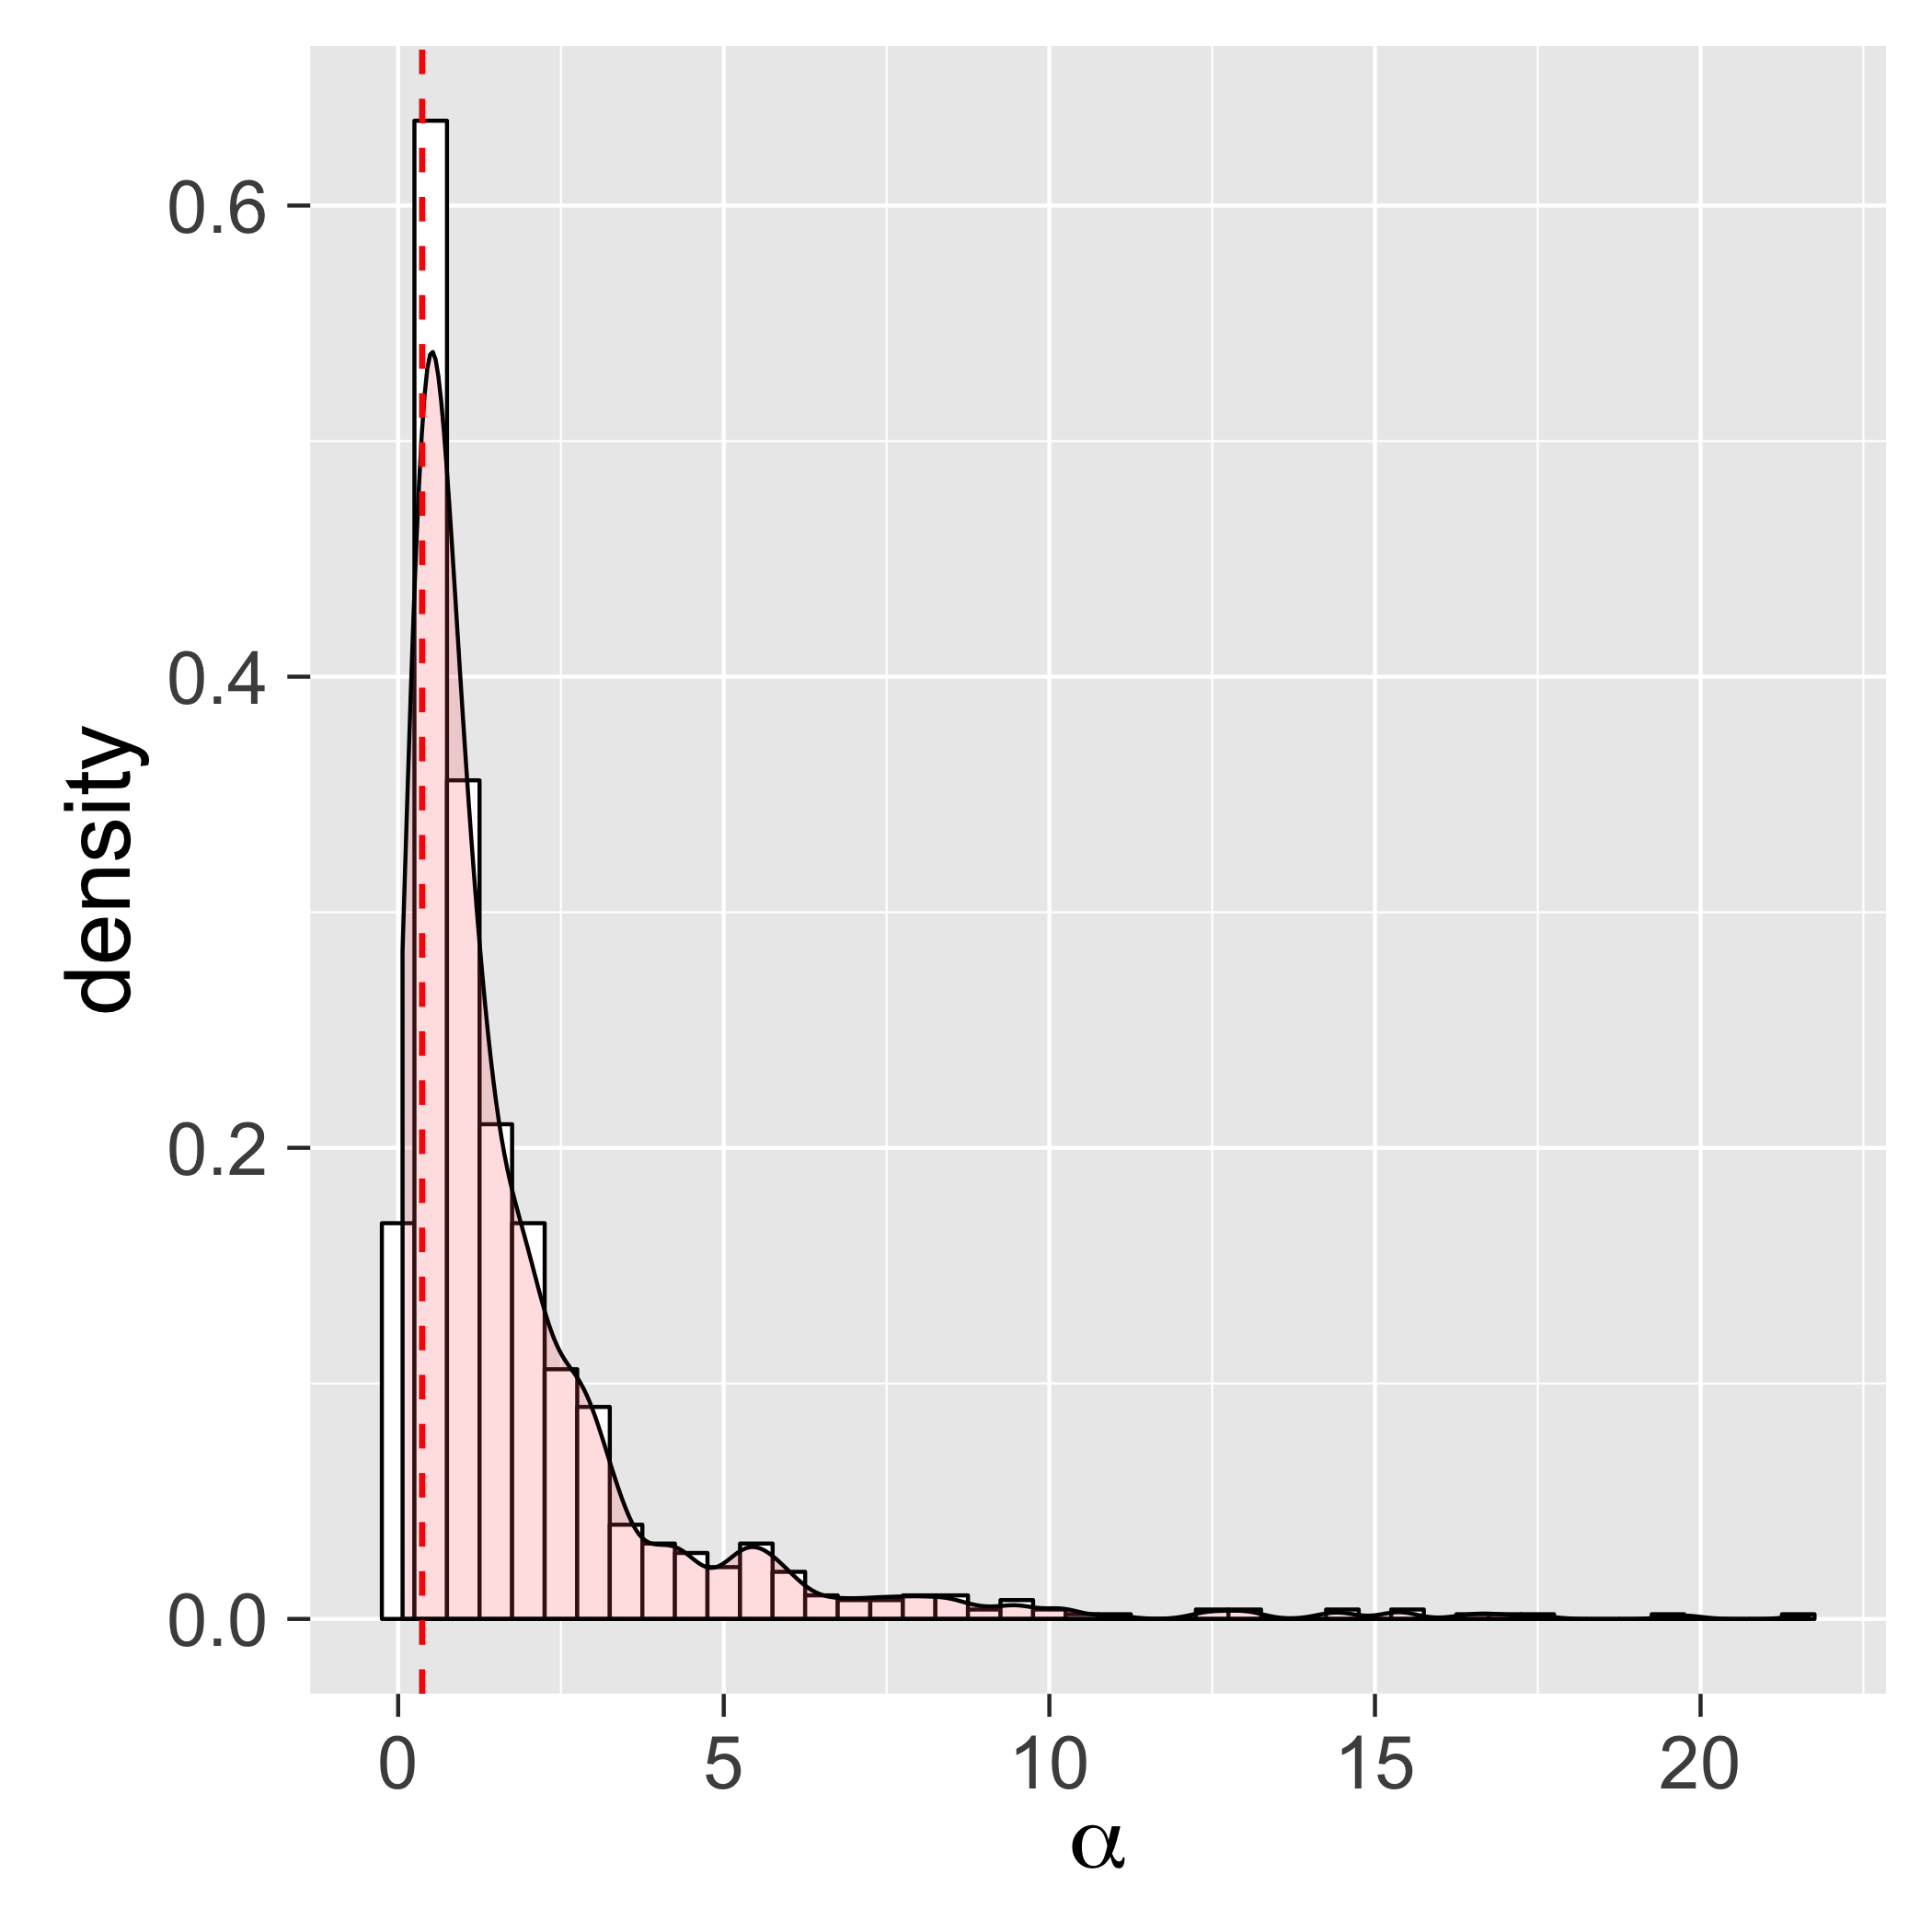
\includegraphics[width=0.4\textwidth]{histogram_alpha_posterior}
  \caption{Posterior Samples $\alpha$}
  \label{fig:alpha}
\end{figure}

\begin{figure}[h]
  \centering
  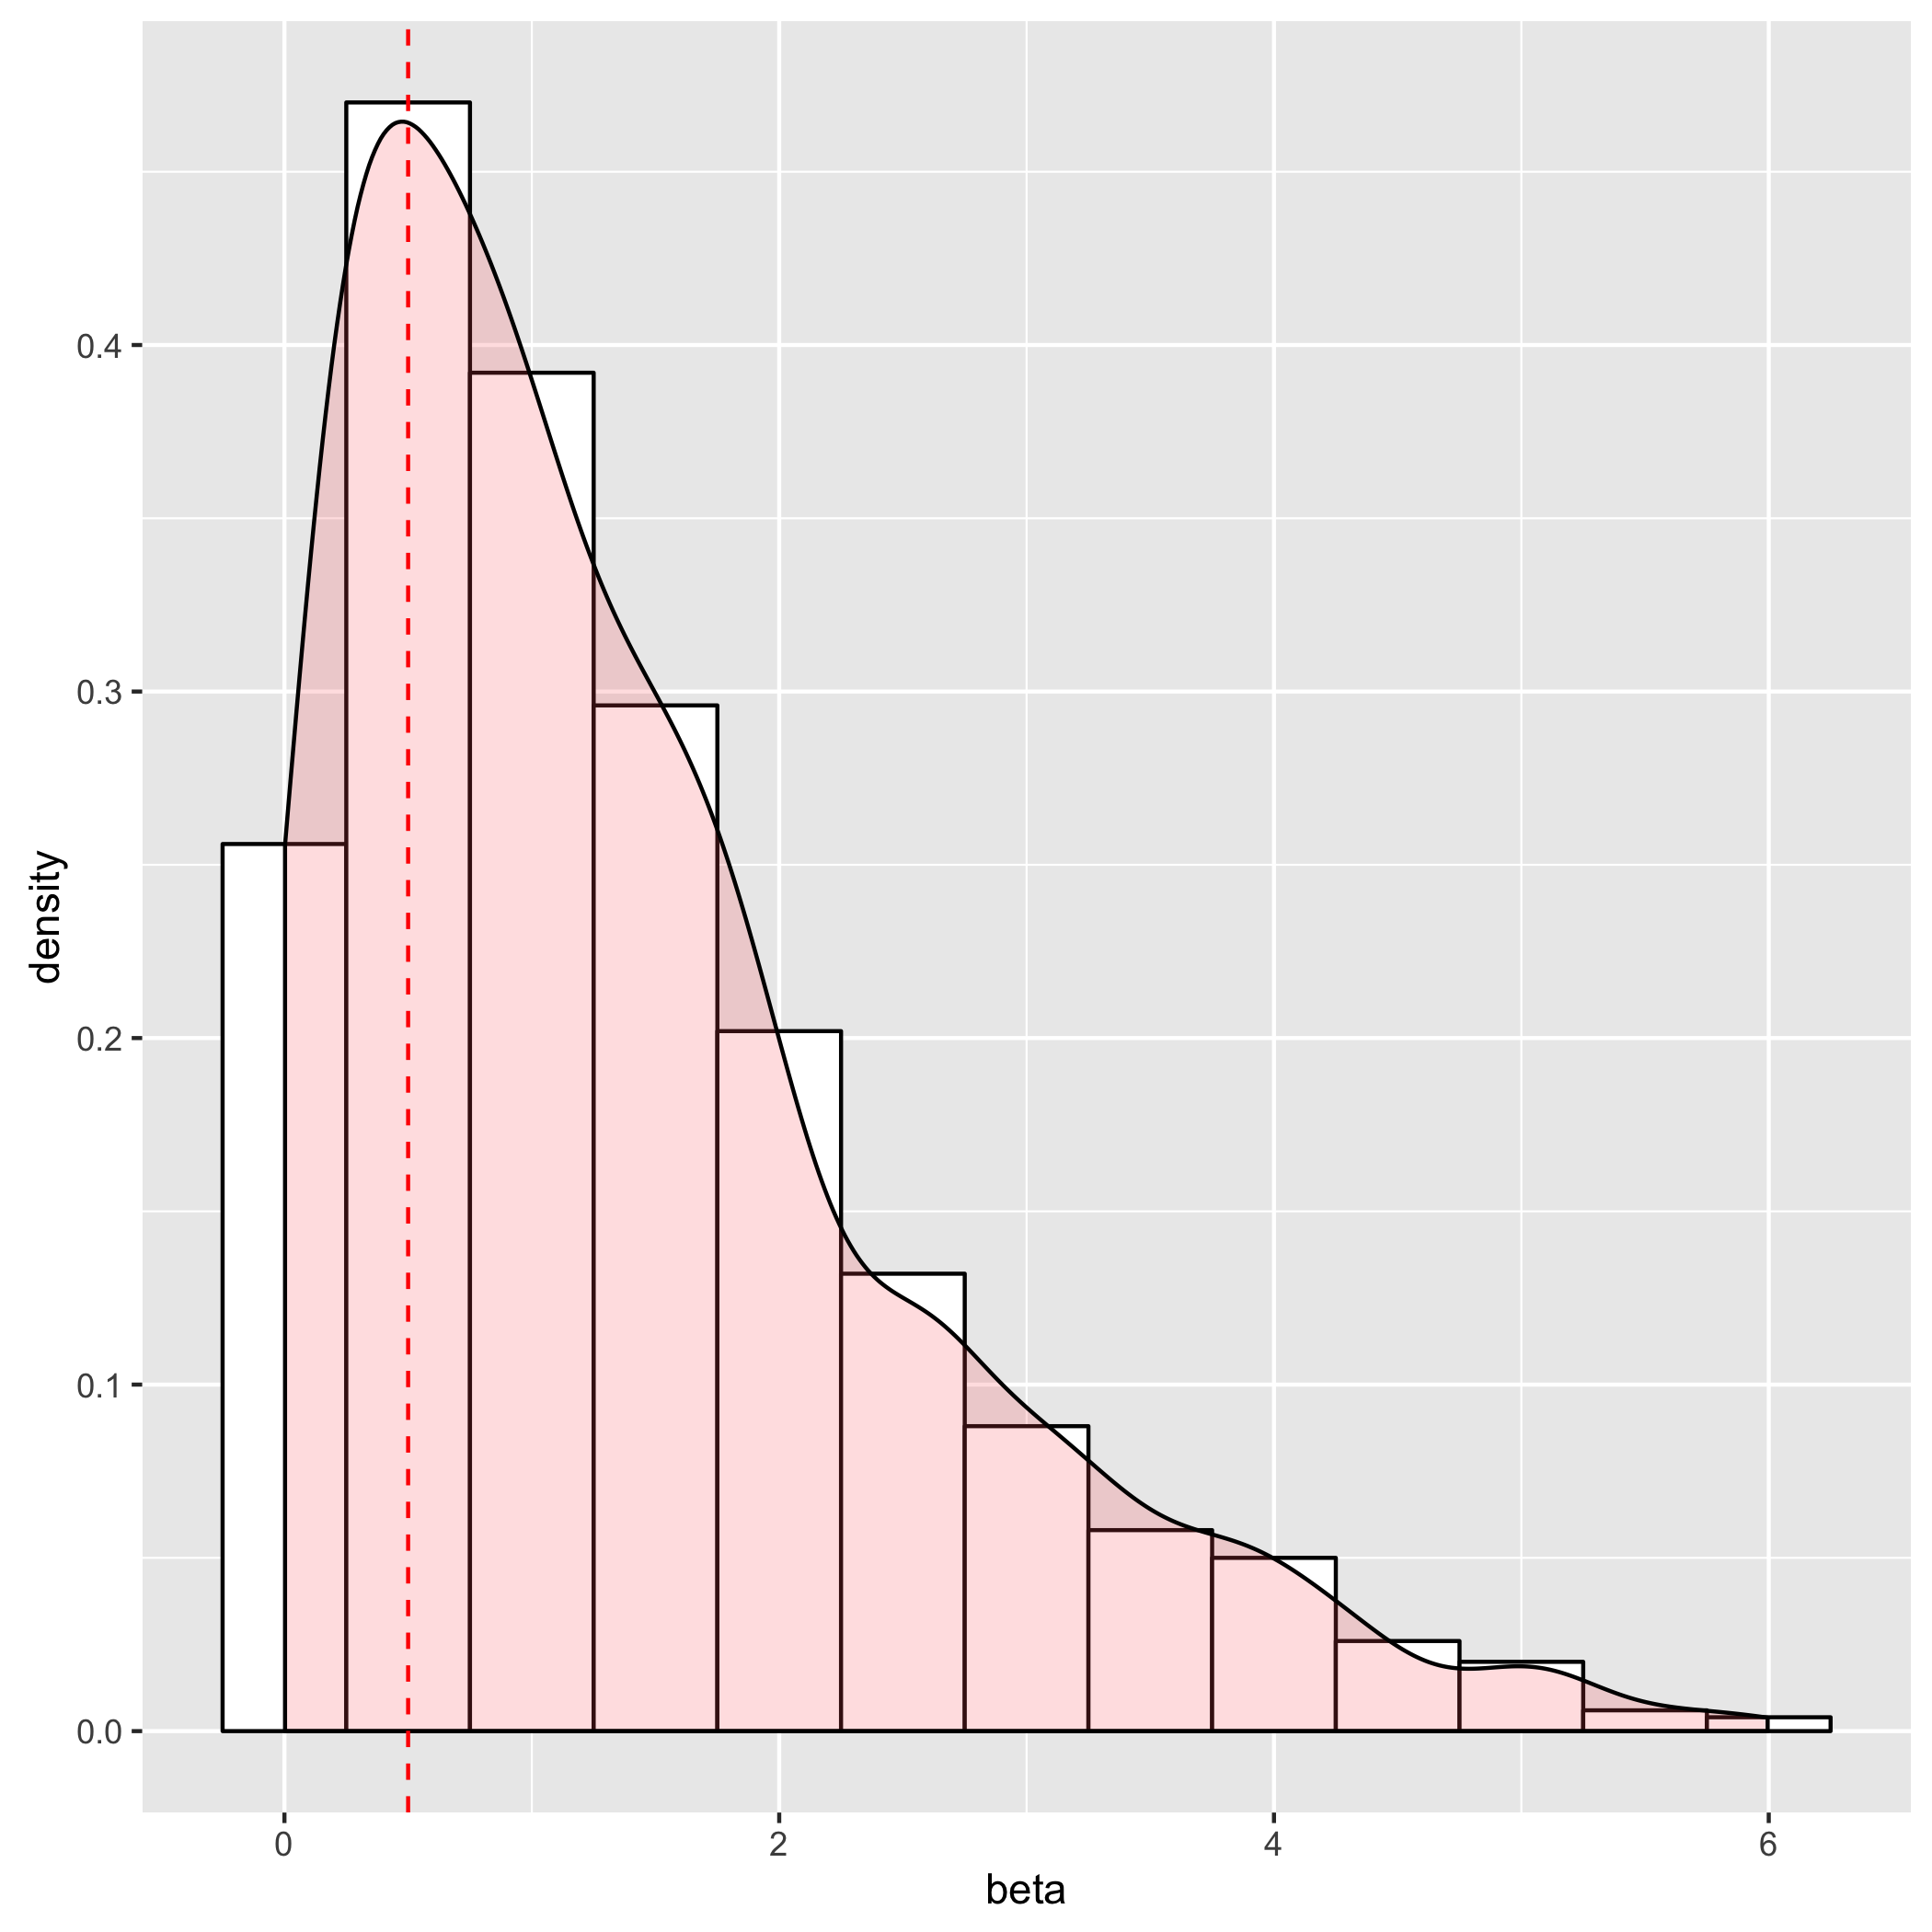
\includegraphics[width=0.4\textwidth]{histogram_beta_posterior}
  \caption{Posterior Samples $\beta$}
  \label{fig:beta}
\end{figure}

\begin{figure}[h]
  \centering
  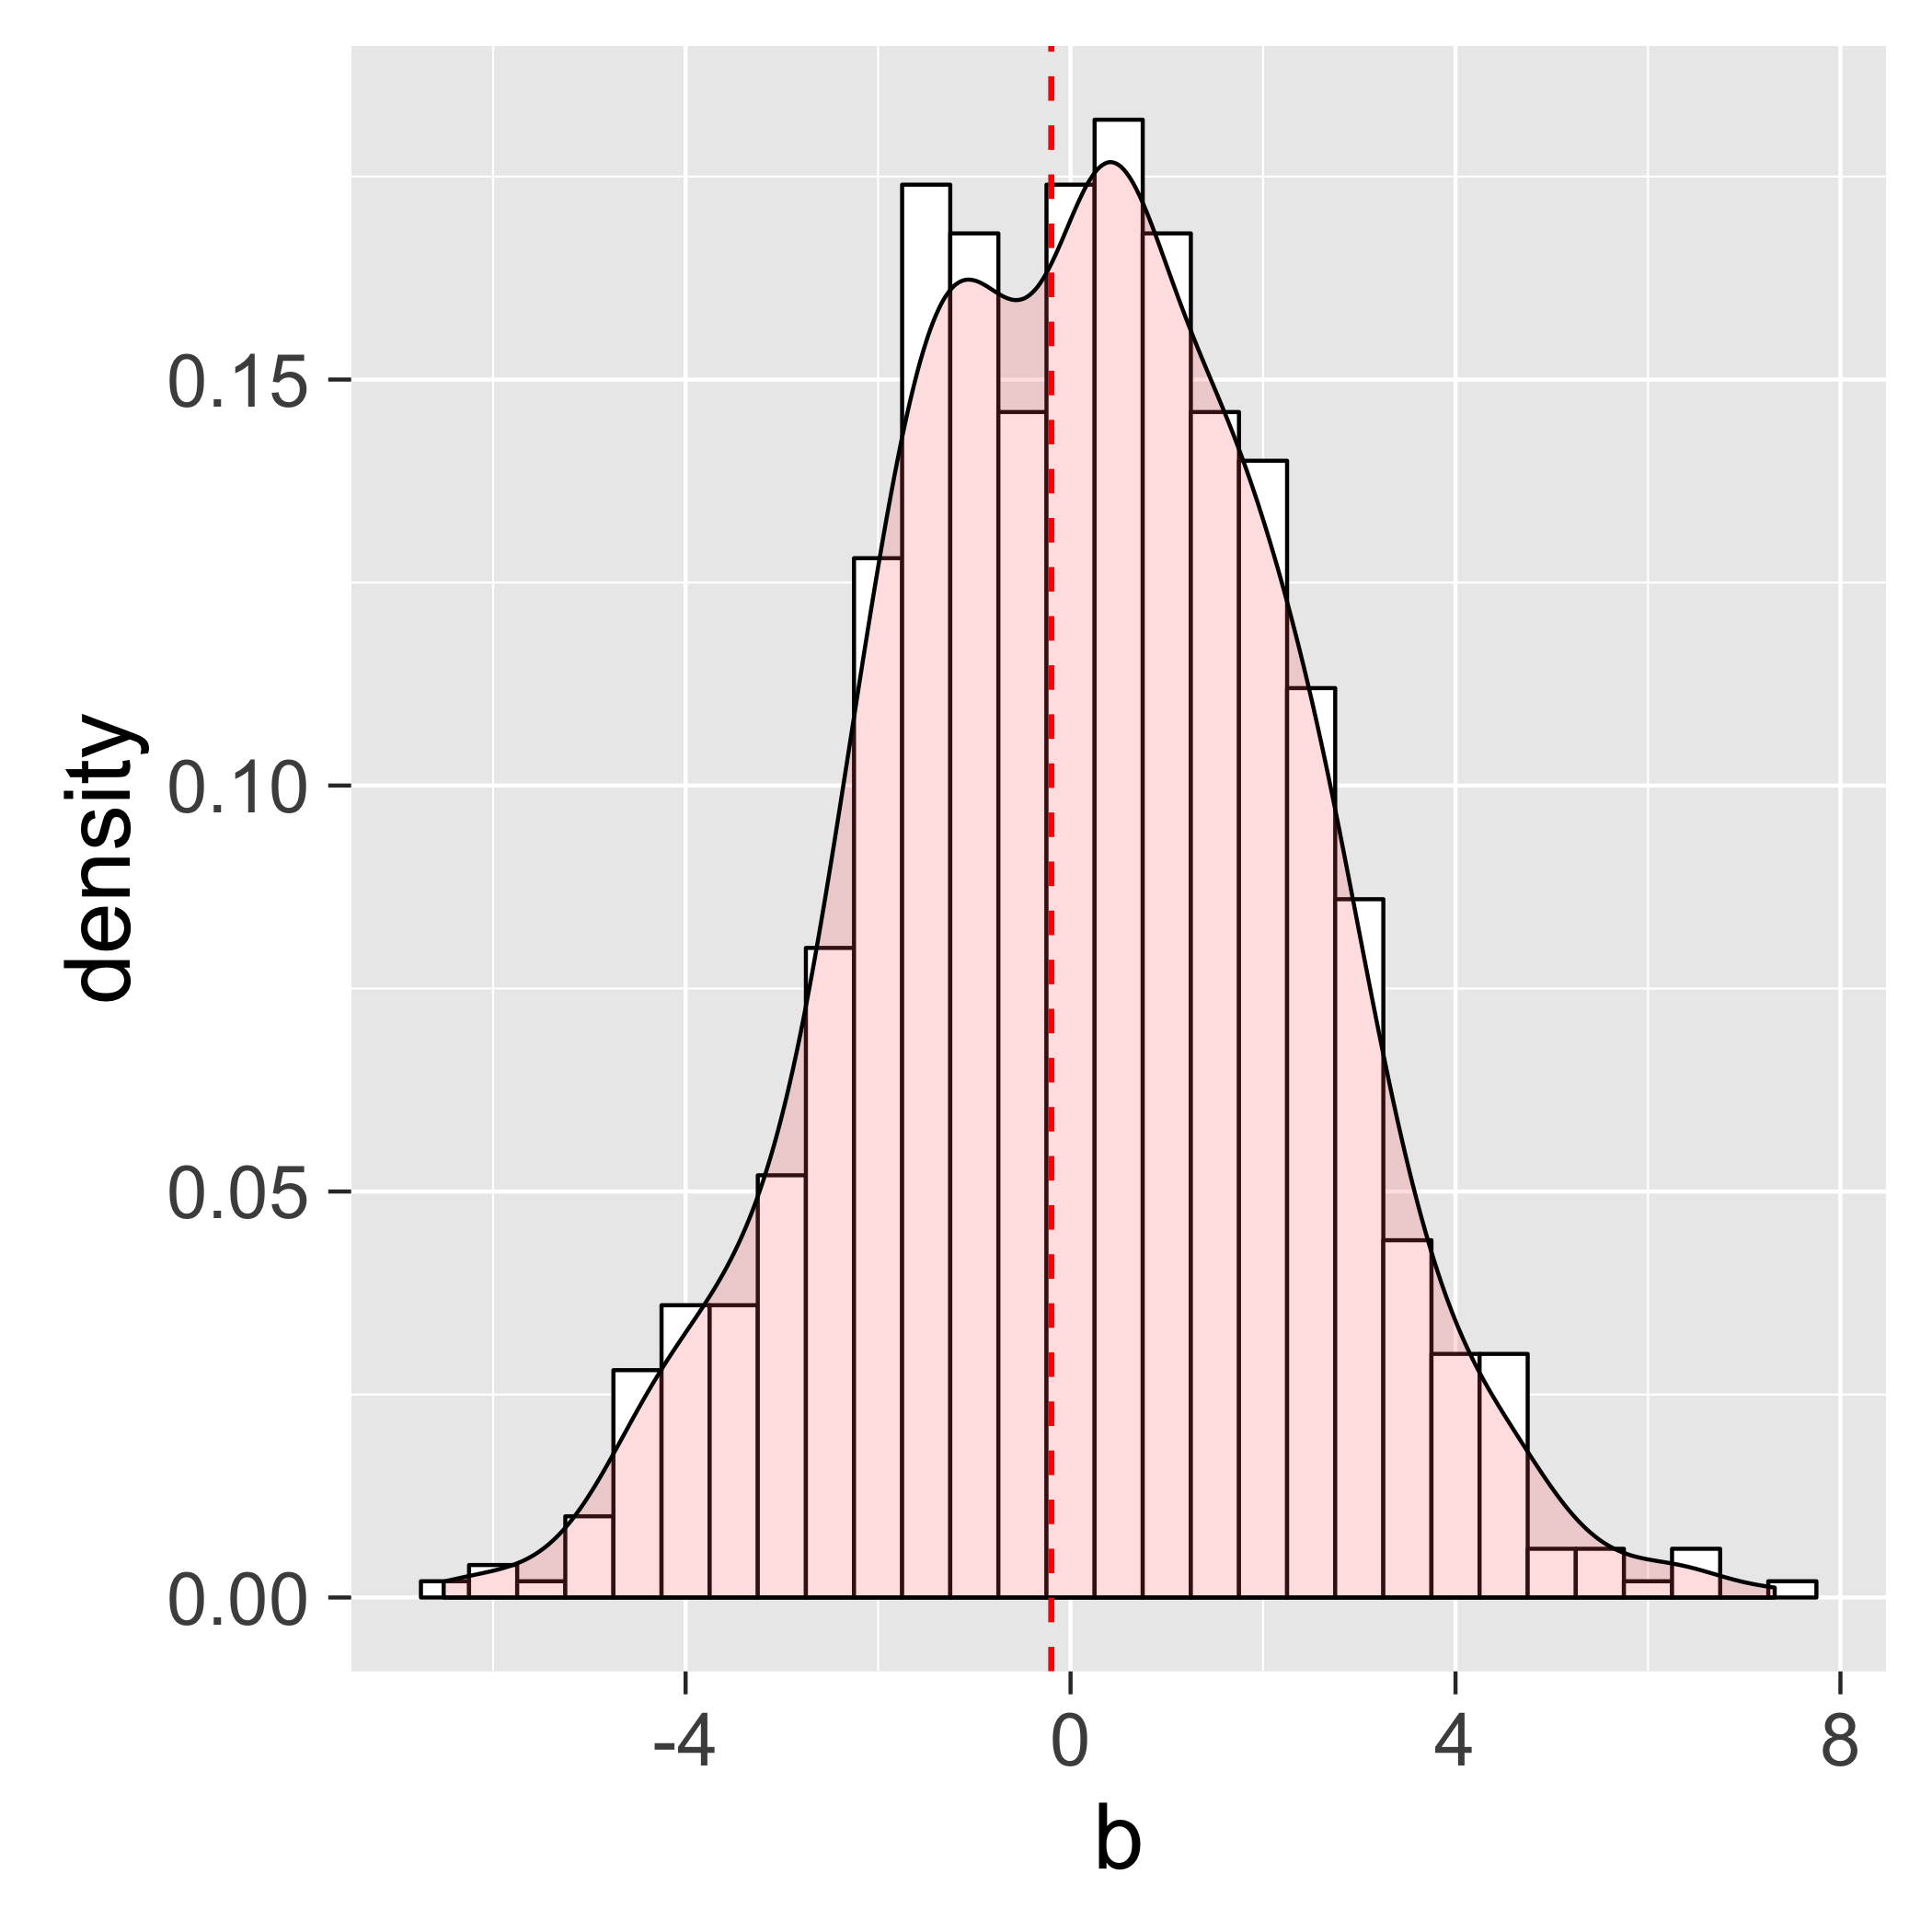
\includegraphics[width=0.4\textwidth]{histogram_b_posterior}
  \caption{Posterior Samples $b$}
  \label{fig:b}
\end{figure}

\subsubsection*{Acknowledgments}

The authors would like to acknowledge travel grant.

\medskip

\small

\bibliography{references}
\end{document}
